\ifspanish

TBD

\else

Let ${X_k, k \ge 0}$ be a Markov chain with state space ${\cal Z} = \{0, 1\}$ and transition probabilities $P\{X_k=1 | X_{k-1}=0\} = 0.8$ and $P\{X_k=0 | X_{k-1}=1\} = 0.4$.

\begin{parts}
\part Draw the corresponding transition graph
\part Assume that the initial state is  $X_0 = 1$. Compute $P\{X_2=1\}$
\part Compute the stationary distribution.
\end{parts}

\begin{solution}
\begin{parts}
\part The transition matrix is 
$$
{\bf P} = \begin{pmatrix}
0.2 & 0.8 \\
0.4 & 0.6
\end{pmatrix}
$$
and, thus, the transition graph is

{\centering
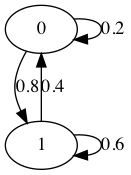
\includegraphics[scale=0.3]{db/figs/MPbinary.png}}

\part 
$$
P\{X_2=1\} = 
    \begin{pmatrix} 0 & 1 \end{pmatrix}
    {\bf P}^\intercal{\bf P}^\intercal
    \begin{pmatrix} 0 \\ 1 \end{pmatrix} 
    = 0.68
$$ 
\part The stationary distribution is the solution of
$$
{\bf P}^\intercal \boldsymbol{\pi} = \boldsymbol{\pi}
$$ 
with $(1, 1) \boldsymbol{\pi} = 1$, that is:
$$
0.2 \pi_0 + 0.4 \pi_1 = \pi_0
$$
and taking $\pi_1 = 1-\pi_0$, we get
$$
0.4 (1-\pi_0)  = 0.8 \pi_0
$$
so that $\pi_0 = \frac13$  and
$$
(\pi_0, \pi_1) = \left(\dfrac13, \dfrac23\right)
$$
\end{parts}
\end{solution}

\fi